
% 4. Docker security
%     1. UID 0
%     2. Privileged Containers
%     3. Secure Computing Mode
%     4. SElinux and AppArmor
\section{Docker Security}
\label{sec::security}

\placeholder{Add security intro}

\subsection{cgroups}
\label{ssec::security:cgroups}

Docker relies on cgroups to limit a container's resources, such as memory, swap, \acs{CPU}, storage and network I/O. cgroups are built into the Linux kernel and this mechanism assures that one container process can't affect the performance of the other processes running on the host machine. In the official kernel documentation it is defined as:
\begin{displayquote}
    \textit{"A mechanism for aggregating/partitioning sets of tasks and all their future children into hierarchical groups with specialized behavior."}
\end{displayquote}
This hierarchy can be displayed in the figure \ref{fig:cgroup-hch}.

\begin{figure}[!htb]
    \centering
    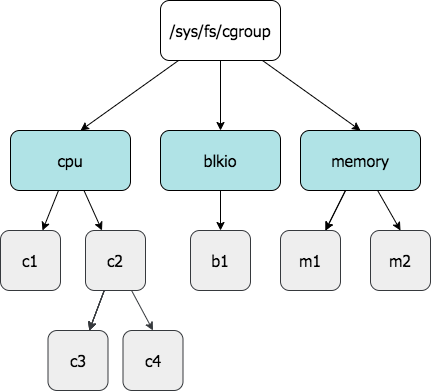
\includegraphics[width=0.25\textwidth]{cgroup.png}
    \caption{Scheme representing Linux cgroup hierarchy\cite{fig-src:cgroups}. Here, the \acs{CPU} resources are split across two tasks, the latter having two child processes. The process \texttt{c3}, for instance, cannot access resources allocated for neither \texttt{c4} or \texttt{c1}. It is constrained to the resources inherited from \texttt{c2}.}
    \label{fig:cgroup-hch}
\end{figure}

When a container is created, Docker automatically assigns a cgroup unique to that container and all the processes of that container will be in the same group.

Constraining resources protects against a class of attacks that attempt to disrupt the system by consuming excessive resources, starving the legitimate applications. It's recommended to set CPU and memory limits in each container when deploying container applications.


\subsection{Namespaces}
\label{ssec::security:namespaces}

A Linux namespace groups a set of global resources in a layer of abstraction so to appear that the processes wrapped in that namespace do not affect the resources not encompassed in that namespace. A process running in a given namespace cannot see or use the resources out of the boundaries set by that namespace.

This tool is the very core of containerization. It allows Docker to divide the \ac{OS} so it appears multiple isolated \acp{OS}. Rather than having a single namespace, Docker containers set up a namespace for each of the six types of resources, these being:

\begin{itemize}
    \item \textbf{\ac{PID} namespace} --- Docker creates \ac{PID} namespace to provide isolated process trees for each container;
    \item \textbf{Mount namespace} --- Each container contains it's own isolated root \texttt{\textbackslash} filesystem. Each process can only access its own isolated mount namespace;
    \item \textbf{\ac{IPC} namespace} --- Allows Docker to manage shared memory both within and outside the container;
    \item \textbf{User namespaces} --- Docker is able to map container users to different users on the Linux host;
    \item \textbf{\ac{UTS} namespace} --- Gives the container its own hostname and domain name. By providing a process running within the container its own \ac{UTS}, it's possible to change the host name of that process without affecting the rest of the system;
    \item \textbf{Network namespace} --- Each container is provided their own isolated network stack, including \acs{IP} address, port ranges and routing table.
\end{itemize}


\subsection{Secure Computing Mode}
\label{ssec::security:sec-compt}

Seccomp (short for secure computing mode) is a Linux mechanism that filters the system calls an application is allowed to make. Each process in seccomp mode is applied a profile that determines what action must be taken when a give system call is matched to the process' profile. When a action is matched, it can either return an error, terminate the process or call a tracer.

Docker applies a default seccomp profile that blocks more than 40 system calls that are undesirable to have a container execute. For instance, a container shouldn't be able to alter the host's clock, so Docker's profile blocks the \texttt{clock\_adjtime} and \texttt{clock\_settime} calls \cite{Rice2020-kl}.

The complete list of system calls can be found in Docker's documentation \cite{docker-seccomp}.


\subsection{Mandatory Access Control}
\label{ssec::security:sel-apparm}

Mandatory Access Control is a class of security system where a system wide security policy grants users access to a given resource. This mechanism gives the administrator more granular control over their system in a way individual users can't override.

Docker supports two major Linux Mandatory Access Control technologies, these being AppArmor and SELinux.

\subsubsection{\textbf{AppArmor}}

One of the \ac{LSM} available in the Linux kernel where an executable file can be associated with a profile, defining what that file is allowed to access. It also allows any violations to logged \cite{ubuntu-apparmor}. A default profile is automatically applied to containers, it provides a wide application compatibility and moderate protection \cite{docker-apparmor}.

\subsubsection{\textbf{SELinux}}
\placeholder{Begin draft}
SElinux lets you constrain what a process is allowed to do in terms of its interactions with files and other processes. Each process runs under an SELinux domain and every file has a type.

Creating an effective SELinux profile for an application takes in-depth knowledge of the set of files that it might need access to, in both happy and error paths, so that task may be best left to the app developer. Some vendors provide profiles for their applications.

\placeholder{End draft}